\documentclass[submit]{harvardml}

\course{CS181-S22}
\assignment{Assignment \#6}
\duedate{11:59PM EST, April 29 2022}
\newcommand{\attr}[1]{\textsf{#1}}
\usepackage[OT1]{fontenc}
\usepackage{float}
\usepackage[colorlinks,citecolor=blue,urlcolor=blue]{hyperref}
\usepackage[pdftex]{graphicx}
\usepackage{subfig}
\usepackage{fullpage}
\usepackage{amsmath}
\usepackage{amssymb}
\usepackage{color}
\usepackage{todonotes}
\usepackage{listings}
\usepackage{common}
\usepackage{bm}
\usepackage{enumitem}
\usepackage{tikz}
\usetikzlibrary{positioning,shapes,arrows}
\usepackage{xifthen}
\usepackage{soul}
\usepackage{framed}
\usepackage{pythonhighlight}

\usepackage[mmddyyyy,hhmmss]{datetime}

\definecolor{verbgray}{gray}{0.9}

\lstnewenvironment{csv}{
  \lstset{backgroundcolor=\color{verbgray},
  frame=single,
  framerule=0pt,
  basicstyle=\ttfamily,
  columns=fullflexible}}{}

\newcommand{\mueps}{\mu_{\epsilon}}
\newcommand{\sigeps}{\sigma_{\epsilon}}
\newcommand{\mugam}{\mu_{\gamma}}
\newcommand{\siggam}{\sigma_{\gamma}}
\newcommand{\muzp}{\mu_{p}}
\newcommand{\sigzp}{\sigma_{p}}
\newcommand{\gauss}[3]{\frac{1}{2\pi#3}e^{-\frac{(#1-#2)^2}{2#3}}}


\begin{document}
\begin{center}
{\Large Homework 6: Inference in Graphical Models, MDPs}\\
\end{center}

\subsection*{Introduction}

In this assignment, you will practice inference in graphical models as
well as MDPs/RL.  For readings, we recommend \href{http://incompleteideas.net/book/the-book-2nd.html}{Sutton and Barto 2018, Reinforcement Learning: An Introduction}, \href{https://harvard-ml-courses.github.io/cs181-web-2017/}{CS181 2017 Lecture Notes}, and Section 10 and 11 Notes.

Please type your solutions after the corresponding problems using this
\LaTeX\ template, and start each problem on a new page.

Please submit the \textbf{writeup PDF to the Gradescope assignment `HW6'}. Remember to assign pages for each question.

Please submit your \textbf{\LaTeX\ file and code files to the Gradescope assignment `HW6 - Supplemental'}. 

You can use a \textbf{maximum of 2 late days} on this assignment.  Late days will be counted based on the latest of your submissions. 
\\

\newpage

\begin{problem}[Explaining Away + Variable Elimination 15 pts]

  In this problem, you will carefully work out a basic example with
  the ``explaining away'' effect. There are many derivations of this
  problem available in textbooks. We emphasize that while you may
  refer to textbooks and other online resources for understanding how
  to do the computation, you should do the computation below from
  scratch, by hand.

  We have three binary variables: rain $R$, wet grass $G$, and
  sprinkler $S$.
We  assume the following factorization of the joint distribution:
$$
\Pr(R,S,G) = \Pr(R)\Pr(S)\Pr(G\, |\, R, S).
  $$
  
  The conditional probability tables look like the
  following:
  \begin{eqnarray*}
    \Pr(R = 1) &= 0.25 \\
    \Pr(S = 1) &= 0.5 \\
    \Pr(G = 1 | R = 0 , S = 0 ) &= 0 \\
    \Pr(G = 1 | R = 1 , S = 0 ) &= .75 \\
    \Pr(G = 1 | R = 0 , S = 1 ) &= .75 \\
    \Pr(G = 1 | R = 1 , S = 1 ) &= 1
  \end{eqnarray*}
  
 
  \begin{enumerate}
    \item Draw the graphical model corresponding to the
      factorization. Are $R$ and $S$ independent?  [Feel free to use
      facts you have learned about studying independence in graphical models.]
    \item You notice it is raining and check on the sprinkler without
      checking the grass.  What is the probability that it is on?
    \item You notice that the grass is wet and go to check on the
      sprinkler (without checking if it is raining).  What is the
      probability that it is on?
    \item You notice that it is raining and the grass is wet.  You go
      check on the sprinkler.  What is the probability that it is on?
    \item What is the ``explaining away'' effect that is shown above?
    \end{enumerate}
    
Consider if we introduce a new binary variable, cloudy $C$, to the the original three binary variables such that the factorization of the joint distribution is now: 

$$
\Pr(C, R,S,G) = \Pr(C)\Pr(R|C)\Pr(S|C)\Pr(G\, |\, R, S).
$$

\begin{enumerate}
    \setcounter{enumi}{5}
    \item For the marginal distribution $\Pr(R)$, write down the variable elimination expression with the elimination ordering $S, G, C$ (where $S$ is eliminated first, then $G$, then $C$).
    \item For the marginal distribution $\Pr(R)$, write down the variable elimination expression with the elimination ordering $C,G,S$.
    \item Give the complexities for each ordering. Which elimination ordering takes less computation?
\end{enumerate}
\end{problem}

%%%%%%%%%%%%%%%%%%%%%%%%%%%%%%%%%%%%%%%%%%%%%%%%%%%%%%%%%%%%%%%%%%%%%%%%%%%%%%%%%%%%%%%%%%%%%%%%%%%%%%%%%%%%%%%%%%%%%%%%%%%%%%%%%%%%%%%
\newpage
\subsection*{Problem 1.1}
We want to draw the graphical model corresponding to the factorization. See the figure below.

\begin{center}
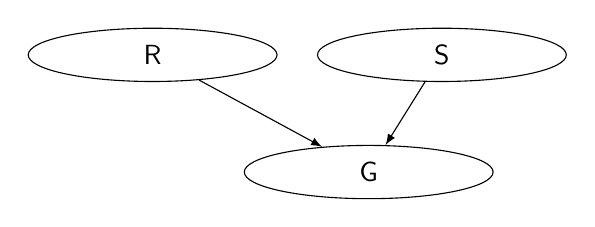
\begin{tikzpicture}[
          node distance=1cm and .5cm,
          bn/.style={draw,ellipse,text width=2cm,align=center}
            ]
    \node[bn] (r) {\attr{R}};
    \node[bn,below right=of r] (g) {\attr{G}};
    \node[bn,right=of r] (s) {\attr{S}};
    \path (r) edge[-latex] (g)
    (s) edge[-latex] (g);
\end{tikzpicture}
\end{center}

$R$ and $S$ are conditionally dependent only given that $G$ is unobserved.

\subsection*{Problem 1.2}
We want to find the probability that the sprinkler is on given that it is raining (we have not checked the grass). This is equivalent to the following.
\begin{align*}
    \Pr(S = 1 | R = 1) &= \frac{\Pr(S = 1, R = 1)}{\Pr(R = 1)}\\
\end{align*}
Let us deal with the joint probability first.
\begin{align*}
    \Pr(S = 1, R = 1) &= \Pr(R = 1)\Pr(S = 1)\Pr(G = 0\, |\, R = 1, S = 1) + \Pr(R = 1)\Pr(S = 1)\Pr(G = 1\, |\, R = 1, S = 1)\\
    &= (0.25) (0.5) (0) + (0.25) (0.5) (1)\\
    &= 0.125
\end{align*}
Then we sub this back in.
\begin{align*}
    \Pr(S = 1 | R = 1) &= \frac{0.125}{0.25}\\
    &= 0.5
\end{align*}
And so this probability is $\boxed{0.5}$.

\subsection*{Problem 1.3}
We want to find the probability that the sprinkler is on given that the grass is wet (without checking the rain). This is equivalent to the following.
\begin{align*}
    \Pr(S = 1 | G = 1) &= \frac{\Pr(S = 1, G = 1)}{\Pr(G = 1)}\\
\end{align*}
Let us deal with the joint probability first.
\begin{align*}
    \Pr(S = 1, G = 1) &= \Pr(R = 1)\Pr(S = 1)\Pr(G = 1\, |\, R = 1, S = 1) + \Pr(R = 0)\Pr(S = 1)\Pr(G = 1\, |\, R = 0, S = 1)\\
    &= (0.25) (0.75) (1) + (0.75) (0.5) (0.75)\\
    &= 0.40625
\end{align*}
Now we find $\Pr(G = 1)$.
\begin{align*}
    \Pr(G = 1) &= \sum_{R, S} \Pr(R) \Pr(S) \Pr(G = 1 | R, S)\\
    &= (0.75) (0.5) (0) + (0.25) (0.5) (0.75) + (0.75) (0.5) (0.75) + (0.25) (0.5) (1)\\
    &= 0.5
\end{align*}
Then we sub these results back in.
\begin{align*}
    \Pr(S = 1 | R = 1) &= \frac{0.40625}{0.5}\\
    &= 0.8125
\end{align*}
And so this probability is $\boxed{0.8125}$.

\subsection*{Problem 1.4}
We want to find the probability that the sprinkler is on given that it is raining and the grass is wet.
\begin{align*}
    \Pr(S = 1 | G = 1, R = 1) &= \frac{\Pr(S = 1, G = 1, R = 1)}{\Pr(G = 1, R = 1)}
\end{align*}
Let us deal with the numerator first.
\begin{align*}
    \Pr(S = 1, G = 1, R = 1) &= \Pr(R = 1)\Pr(S = 1)\Pr(G = 1\, |\, R = 1, S = 1)
    &= (0.25) (0.5) (1)\\
    &= 0.125
\end{align*}
Then we deal with the denominator.
\begin{align*}
    \Pr(G = 1, R = 1) &= \sum_{S} \Pr(S, G = 1, R = 1)\\
    &= \sum_{S} \Pr(R = 1)\Pr(S)\Pr(G = 1 | R = 1, S)\\
    &= (0.25) (0.5) (0.75) + (0.5) (0.25) (1)\\
    &= 0.21875
\end{align*}
Then we sub these results back in.
\begin{align*}
    \Pr(S = 1 | G = 1, R = 1) &= \frac{0.125}{0.21875}\\
    &= 0.571
\end{align*}
And so this probability is $\boxed{0.571}$.

\subsection*{Problem 1.5}
The above probabilities show an explaining away effect. As we can see, $\Pr(S = 1 | G = 1) < \Pr(S = 1 | G = 1, R = 1)$: the probability that the sprinkler is on given that the grass is wet is lower than the probability that the sprinkler given that the grass is wet and it is raining. This makes sense, because the fact that it is raining ``explains'' that the grass is wet, making it less likely that the sprinkler is on.

\subsection*{Problem 1.6}
We want to write down the variable expression with ordering $S, G, C$ for the marginal distribution $\Pr(R)$.
\begin{align*}
    \Pr(R) &= \sum_{C} \sum_{G} \sum_{S} \Pr(C) \Pr(R | C) \Pr(S | C) \Pr(G | R, S)\\
    &= \sum_{C} \Pr(C) \Pr(R | C) \sum_{G} \sum_{S} \Pr(S | C) \Pr(G | R, S)\\
    &= \sum_{C} \Pr(C) \Pr(R | C) \sum_{G} \phi_1(C, G, R) \\
    &= \sum_{C} \Pr(C) \Pr(R | C) \phi_2(C, R) \\
    &= \phi_3(R)
\end{align*}

\subsection*{Problem 1.7}
We want to write down the variable expression with ordering $C, G, S$ for the marginal distribution $\Pr(R)$.
\begin{align*}
    \Pr(R) &= \sum_{S} \sum_{G} \sum_{C} \Pr(C) \Pr(R | C) \Pr(S | C) \Pr(G | R, S)\\
    &= \sum_{S} \sum_{G} \Pr(G | R, S) \sum_{C} \Pr(C) \Pr(R | C) \Pr(S | C) \\
    &= \sum_{S} \sum_{G} \Pr(G | R, S) \phi_1(R, S) \\
    &= \sum_{S} \phi_1(R, S) \sum_{G} \Pr(G | R, S) \\
    &= \sum_{S} \phi_1(R, S) \phi_2(R, S) \\
    &= \phi_3(R)
\end{align*}

\subsection*{Problem 1.8}
The first ordering (in Problem 1.6) has an innermost term of $\Pr(S|C) \Pr(G | R, S)$ which contains four variables, $S, C, G, R$, and so the complexity is $O(K^4)$ for the $K$ values of $R$. The second ordering has an innermost term of $\Pr(C)\Pr(R | C) \Pr(S | C)$ which contains three variables, $C, R, S$, and so the complexity is $O(K^3)$ for the $K$ values of $R$. And so the second elimination ordering $C, G, S$ takes less computation.


%%%%%%%%%%%%%%%%%%%%%%%%%%%%%%%%%%%%%%%%%%%%%%%%%%%%%%%%%%%%%%%%%%%%%%%%%%%%%%%%%%%%%%%%%%%%%%%%%%%%%%%%%%%%%%%%%%%%%%%%%%%%%%%%%%%%%%%

\newpage
\begin{problem}[Policy and Value Iteration, 15 pts]

This question asks you to implement policy and value iteration in a
simple environment called Gridworld.  The ``states'' in Gridworld are
represented by locations in a two-dimensional space.  Here we show each state and its reward:

\begin{center}
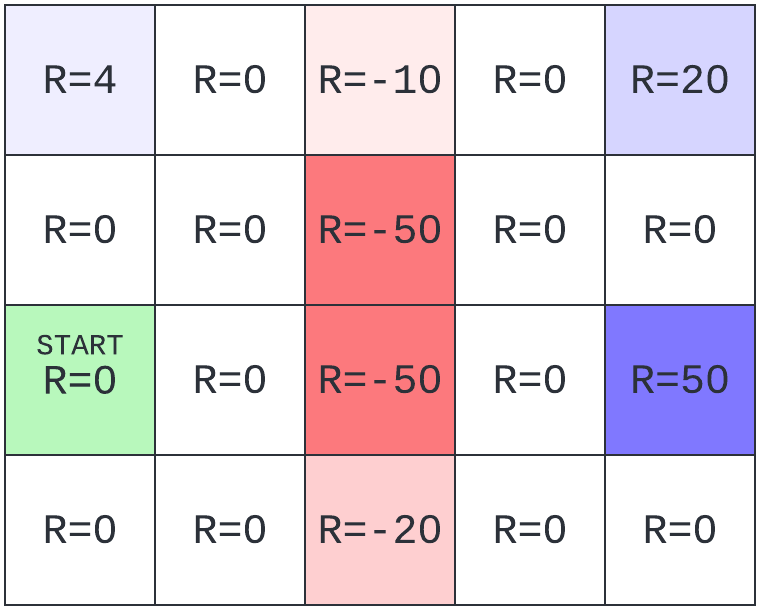
\includegraphics[width=3in]{gridworld.png}
\end{center}
The set of actions is \{N, S, E, W\}, which corresponds to moving north (up), south (down), east (right), and west (left) on the grid.
Taking an action in Gridworld does not always succeed with probability
$1$; instead the agent has probability $0.1$ of ``slipping'' into a
state on either side, but not backwards.  For example, if the agent tries to move right from START, it succeeds with probability 0.8, but the agent may end up moving up or down with probability 0.1 each. Also, the agent cannot move off the edge of the grid, so moving left from START will keep the agent in the same state with probability 0.8, but also may slip up or down with probability 0.1 each. Lastly, the agent has no chance of slipping off the grid - so moving up from START results in a 0.9 chance of success with a 0.1 chance of moving right.

Also, the agent does not receive the reward of a state immediately upon entry, but instead only after it takes an action at that state. For example, if the agent moves right four times (deterministically, with no chance of slipping) the rewards would be +0, +0, -50, +0, and the agent would reside in the +50 state. Regardless of what action the agent takes here, the next reward would be +50.

Your job is to implement the following three methods in file \texttt{T6\_P2.ipynb}. Please use the provided helper functions \texttt{get\_reward} and \texttt{get\_transition\_prob} to implement your solution.

\emph{Do not use any outside code.  (You may still collaborate with others according to the standard collaboration policy in the syllabus.)}  

\emph{Embed all plots in your writeup.}
\end{problem}
\newpage

\begin{framed}
\textbf{Problem 2} (cont.)\\

\textbf{Important: } The state space is represented using integers, which range from 0 (the top left) to 19 (the bottom right). Therefore both the policy \texttt{pi} and the value function \texttt{V} are 1-dimensional arrays of length \texttt{num\_states = 20}. Your policy and value iteration methods should only implement one update step of the iteration - they will be repeatedly called by the provided \texttt{learn\_strategy} method to learn and display the optimal policy. You can change the number of iterations that your code is run and displayed by changing the $\texttt{max\_iter}$ and $\texttt{print\_every}$ parameters of the $\texttt{learn\_strategy}$ function calls at the end of the code.

Note that we are doing infinite-horizon planning to maximize the expected reward of the traveling agent. For parts 1-3, set discount factor $\gamma = 0.7$.

\begin{itemize}
    \item[1a.]  Implement function \texttt{policy\_evaluation}.  Your
      solution should learn value function $V$, either using a closed-form expression or iteratively using
      convergence tolerance $\texttt{theta = 0.0001}$ (i.e., if
      $V^{(t)}$ represents $V$ on the $t$-th iteration of your policy
      evaluation procedure, then if $|V^{(t + 1)}[s] - V^{(t)}[s]|
      \leq \theta$ for all $s$, then terminate and return $V^{(t + 1)}$.)

    \item[1b.] Implement function \texttt{update\_policy\_iteration} to update the policy \texttt{pi} given a value function \texttt{V} using \textbf{one step} of policy iteration.
    
    \item[1c.] Set \texttt{max\_iter = 4}, \texttt{print\_every = 1} to show the learned value function and the associated policy for the first 4 policy iterations. Do not modify the plotting code. Please fit all 4 plots onto one page of your writeup.
    
    \item [1d.] Set \texttt{ct = 0.01} and increase \texttt{max\_iter} such that the algorithm converges. Include a plot of the final learned value function and policy. How many iterations does it take to converge? Now try \texttt{ct = 0.001} and \texttt{ct = 0.0001}. How does this affect the number of iterations until convergence?
      
    \item [2a.] Implement function
      \texttt{update\_value\_iteration}, which performs \textbf{one step} of value iteration to update \texttt{V}, \texttt{pi}.
      
    \item [2b.] Set \texttt{max\_iter = 4}, \texttt{print\_every = 1} to show the learned value function and the associated policy for the first 4 value iterations. Do not modify the plotting code. Please fit all 4 plots onto one page of your writeup.
    
    \item [2c.] Set \texttt{ct = 0.01} and increase \texttt{max\_iter} such that the algorithm converges. Include a plot of the final learned value function and policy. How many iterations does it take to converge? Now try \texttt{ct = 0.001} and \texttt{ct = 0.0001}. How does this affect the number of iterations until convergence?
    
    \item[3] Compare and contrast the number of iterations, time per iteration, and overall runtime between policy iteration and value iteration. What do you notice?
    
    \item[4] Plot the learned policy with each of $\gamma \in (0.6,0.7,0.8,0.9)$. Include all 4 plots in your writeup. Describe what you see and provide explanations for the differences in the observed policies. Also discuss the effect of gamma on the runtime for both policy and value iteration.
    
    \item[5] Now suppose that the game ends at any state with a positive reward, i.e. it immediately transitions you to a new state with zero reward that you cannot transition away from. What do you expect the optimal policy to look like, as a function of gamma? Numerical answers are not required, intuition is sufficient.
 
\end{itemize}
\end{framed}

%%%%%%%%%%%%%%%%%%%%%%%%%%%%%%%%%%%%%%%%%%%%%%%%%%%%%%%%%%%%%%%%%%%%%%%%%%%%%%%%%%%%%%%%%%%%%%%%%%%%%%%%%%%%%%%%%%%%%%%%%%%%%%%%%%%%%%%%%%%%%%%%%%
\newpage
\subsection*{Problem 2.1a}

We want to implement the function \texttt{policy\_evaluation}. We do so iteratively using a threshold of $\theta = 0.0001$. The code is given below.
\begin{python}
def policy_evaluation(pi, gamma):
    theta = 0.0001
    V = np.zeros(num_states)
    diff = float('inf')
    while diff > theta:
        V_k = np.zeros(num_states)
        for s1 in range(num_states):
            expected = 0
            for s2 in range(num_states):
                expected += get_transition_prob(s1, pi[s1], s2) * V[s2]
            V_k[s1] = get_reward(s1) + gamma * expected
        diff = np.max(np.abs(V_k - V))
        V = np.copy(V_k)
    return V
\end{python}

\subsection*{Problem 2.1b}
We want to implement the function \texttt{update\_policy\_iteration} to update the policy given a value function using one step of policy iteration. The code is given below.
\begin{python}
def update_policy_iteration(V, gamma):
    pi_new = np.zeros(num_states)
    for s1 in range(num_states):
        mval = -float('inf')
        for a in range(num_actions):
            expected = 0 
            for s2 in range(num_states):
                expected += get_transition_prob(s1, a, s2) * V[s2]
            cval = get_reward(s1) + gamma * expected
            if cval > mval:
                mval = cval
                pi_new[s1] = a
    return pi_new
\end{python}

\newpage
\subsection*{Problem 2.1c}
We want to plot the learned function and associated policy for the first 4 policy iterations.

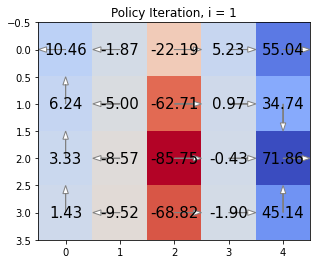
\includegraphics[width=0.5\linewidth]{q2/polit1.png}
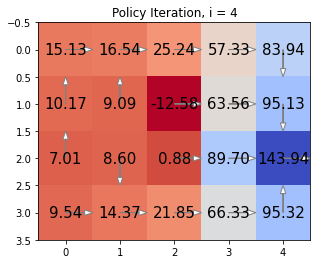
\includegraphics[width=0.5\linewidth]{q2/polit2.png}
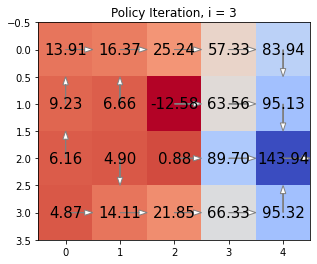
\includegraphics[width=0.5\linewidth]{q2/polit3.png}
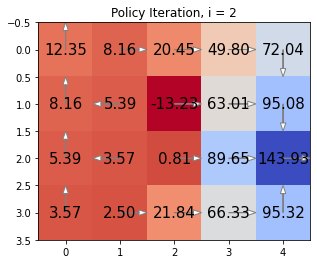
\includegraphics[width=0.5\linewidth]{q2/polit4.png}

\newpage
\subsection*{Problem 2.1d}
We want to plot the final learned value function and policy, setting \texttt{ct = 0.01} and increasing \texttt{max\_iter} to an appropriate number. The final learned value and policy is given below.

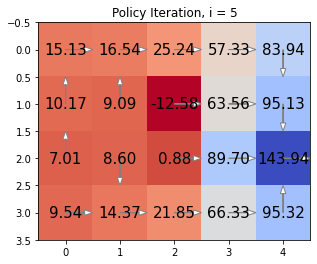
\includegraphics[width=0.5\linewidth]{q2/polit5.png}

This took five iterations to converge. Trying \texttt{max\_iter = 0.001} and \texttt{max\_iter = 0.0001} did not change the number of iterations until convergence.

\subsection*{Problem 2.2a}
We want to implement the function \texttt{update\_value\_iteration}. The code is below.
\begin{python}
def update_value_iteration(V, gamma):
    V_new = np.zeros(num_states)
    pi_new = np.zeros(num_states)
    
    for s1 in range(num_states):
        mvalue = -float('inf')
        for a in range(num_actions):
            expected = 0
            for s2 in range(num_states):
                expected += get_transition_prob(s1, a, s2) * V[s2]
            cvalue = get_reward(s1) + gamma * expected
            if mvalue < cvalue:
                mvalue = cvalue
        V_new[s1] = mvalue

    pi_new = np.zeros(num_states)
    for s1 in range(num_states):
        mval = -float('inf')
        for a in range(num_actions):
            expected = 0 
            for s2 in range(num_states):
                expected += get_transition_prob(s1, a, s2) * V_new[s2]
            cval = get_reward(s1) + gamma * expected
            if cval > mval:
                mval = cval
                pi_new[s1] = a
    
    return V_new, pi_new
\end{python}

\subsection*{Problem 2.2b}
We want to show the learned value function and the associated for the first 4 value iterations.

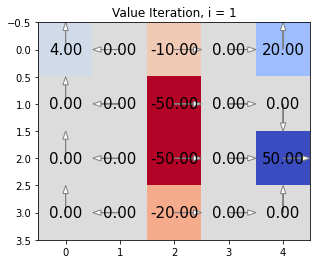
\includegraphics[width=0.5\linewidth]{q2/valit1.png}
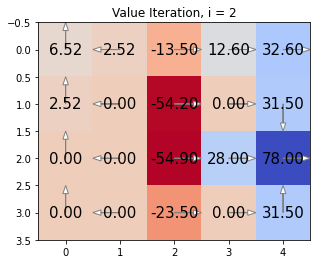
\includegraphics[width=0.5\linewidth]{q2/valit2.png}
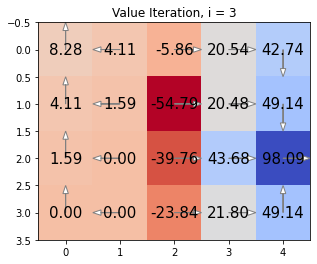
\includegraphics[width=0.5\linewidth]{q2/valit3.png}
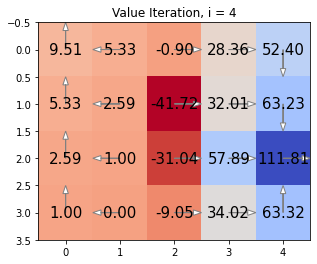
\includegraphics[width=0.5\linewidth]{q2/valit4.png}

\newpage
\subsection*{Problem 2.2c}
We want to plot the final learned value function and policy, setting \texttt{ct = 0.01} and increasing \texttt{max\_iter} to an appropriate number. The final learned value and policy is given below.

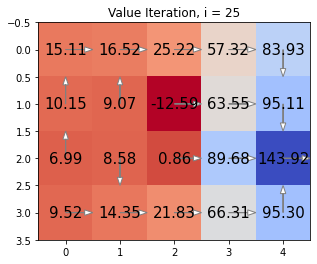
\includegraphics[width=0.5\linewidth]{q2/valit25.png}

Value iteration takes 25 iterations to converge. Setting \texttt{ct = 0.001} requires $21$ iterations to converge, and setting \texttt{ct = 0.0001} requires $38$ iterations to converge. As \texttt{ct} decreases, the number of iterations required for converge increases.

\subsection*{2.3}
Value iteration takes many more iterations to converge than policy iteration. When timing both value and policy iteration, both had an overall runtime of approximately $2.1$ seconds on my machine. This means that value iteration took $2.1 / 25 \approx 0.085$ seconds per iteration whereas policy iteration took $2.1 / 5 = 0.42$ seconds per iteration. So, while policy iteration takes less iterations overall, the increased computational cost of each iteration results in it having approximately the same runtime as value iteration.

\newpage
\subsection*{2.4}
We want to plot the learned policy for each $\gamma \in \{0.6, 0.7, 0.8, 0.9\}$.

First, with policy iteration we get the following plots. The top-left is $\gamma = 0.6$, the top-right is $\gamma =0.7$, the bottom-left is $\gamma = 0.8$, and the bottom-right plot is $\gamma = 0.9.$

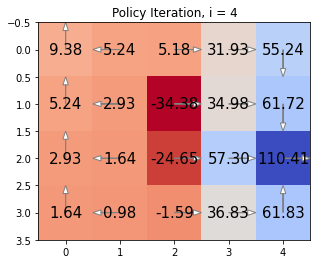
\includegraphics[width=0.5\linewidth]{q2/gammas/polit06.png}
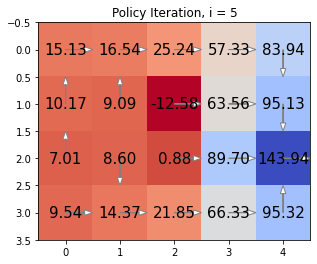
\includegraphics[width=0.5\linewidth]{q2/gammas/polit07.png}
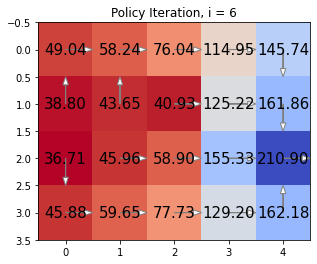
\includegraphics[width=0.5\linewidth]{q2/gammas/polit08.png}
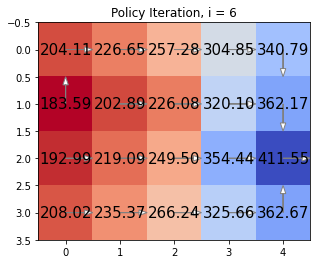
\includegraphics[width=0.5\linewidth]{q2/gammas/polit09.png}

Next, with value iteration, we get the following plots. The ordering of the plots by gammas is the same as that of policy iteration above.

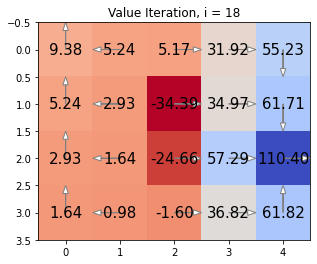
\includegraphics[width=0.5\linewidth]{q2/gammas/valit06.png}
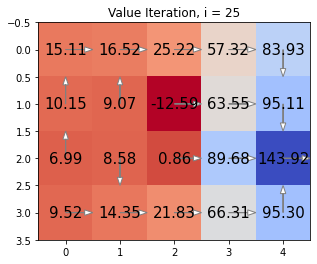
\includegraphics[width=0.5\linewidth]{q2/gammas/valit07.png}
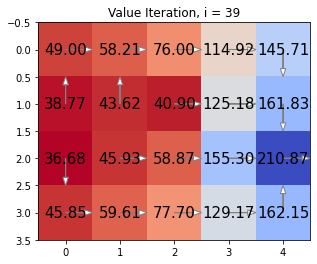
\includegraphics[width=0.5\linewidth]{q2/gammas/valit08.png}
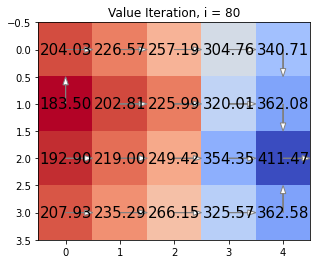
\includegraphics[width=0.5\linewidth]{q2/gammas/valit09.png}

As we can see, for lower values of gamma the converged policy tends to take actions that move toward the closest positive cell. This is because farther positive rewards are discounted below the value of the closer reward. For higher values of gamma, further positive rewards are not as heavily discounted and so the optimal policy is to move in their direction.

For value iteration, as the value of gamma increases the runtime also increases. For policy iteration, as the value of gamma increases the runtime also increases albeit at a much slower rate than for value iteration.

\subsection*{2.5}
We want to discuss the effect of a modification to the game where the game ends at any state with a positive reward on the optimal policy as a function of gamma. As gamma decreases, nearby states are valued more highly than far-away states, and so the optimal policy would favor going to a near-by state and then ending the game. As gamma increases, far-away states are valued around the same as nearby-states, and so the optimal policy would favor the cell with the highest reward regardless of its distance from the current state.

%%%%%%%%%%%%%%%%%%%%%%%%%%%%%%%%%%%%%%%%%%%%%%%%%%%%%%%%%%%%%%%%%%%%%%%%%%%%%%%%%%%%%%%%%%%%%%%%%%%%%%%%%%%%%%%%%%%%%%%%%%%%%%%%%%%%%%%%%%%%%%%%%%

\begin{problem}[Reinforcement Learning, 20 pts]
  In 2013, the mobile game \emph{Flappy Bird} took the world by storm. You'll be developing a Q-learning agent to play a similar game, \emph{Swingy Monkey} (See Figure~\ref{fig:swingy}).  In this game, you control a monkey that is trying to swing on vines and avoid tree trunks.  You can either make him jump to a new vine, or have him swing down on the vine he's currently holding.  You get points for successfully passing tree trunks without hitting them, falling off the bottom of the screen, or jumping off the top.  There are some sources of randomness: the monkey's jumps are sometimes higher than others, the gaps in the trees vary vertically, the gravity varies from game to game, and the distances between the trees are different.  You can play the game directly by pushing a key on the keyboard to make the monkey jump.  However, your objective is to build an agent that \emph{learns} to play on its own. 
  
   You will need to install the \verb|pygame| module
  (\url{http://www.pygame.org/wiki/GettingStarted}).
  

\textbf{Task:}
Your task is to use Q-learning to find a policy for the monkey that can navigate the trees.  The implementation of the game itself is in file \verb|SwingyMonkey.py|, along with a few files in the \verb|res/| directory.  A file called \verb|stub.py| is the starter code for setting up your learner that interacts with the game.  This is the only file you need to modify (but to speed up testing, you can comment out the animation rendering code in \verb|SwingyMonkey.py|). You can watch a YouTube video of the staff Q-Learner playing the game at \url{http://youtu.be/l4QjPr1uCac}.  It figures out a reasonable policy in a few dozen iterations.
You'll be responsible for implementing the Python function  \verb|action_callback|. The action callback will take in a dictionary that describes the current state of the game and return an action for the next time step.  This will be a binary action, where 0 means to swing downward and 1 means to jump up.  The dictionary you get for the state looks like this:
\begin{csv}
{ 'score': <current score>,
  'tree': { 'dist': <pixels to next tree trunk>,
            'top':  <height of top of tree trunk gap>,
            'bot':  <height of bottom of tree trunk gap> },
  'monkey': { 'vel': <current monkey y-axis speed>,
              'top': <height of top of monkey>,
              'bot': <height of bottom of monkey> }}
\end{csv}
All of the units here (except score) will be in screen pixels. Figure~\ref{fig:swingy-ann} shows these graphically. 
Note that since the state space is very large (effectively continuous), the monkey's relative position needs to be discretized into bins. The pre-defined function \verb|discretize_state| does this for you.

\textbf{Requirements}
\\
\textit{Code}: First, you should implement Q-learning with an
$\epsilon$-greedy policy yourself. You can increase the performance by
trying out different parameters for the learning rate $\alpha$,
discount rate $\gamma$, and exploration rate $\epsilon$. \emph{Do not use outside RL code for this assignment.} Second, you should use a method of your choice to further improve the performance. This could be inferring gravity at each epoch (the gravity varies from game to game), updating the reward function, trying decaying epsilon greedy functions, changing the features in the state space, and more. One of our staff solutions got scores over 800 before the 100th epoch, but you are only expected to reach scores over 50 before the 100th epoch. {\bf Make sure to turn in your code!} \\\\
\textit{Evaluation}: In 1-2 paragraphs, explain how your agent performed and what decisions you made and why. Make sure to provide evidence where necessary to explain your decisions. You must include in your write up at least one plot or table that details the performances of parameters tried (i.e. plots of score vs. epoch number for different parameters).
\\\\
\textit{Note}: Note that you can simply discretize the state and action spaces and run the Q-learning algorithm. There is no need to use complex models such as neural networks to solve this problem, but you may do so as a fun exercise.

\end{problem}
\begin{figure}[H]
    \centering%
    \subfloat[SwingyMonkey Screenshot]{%
        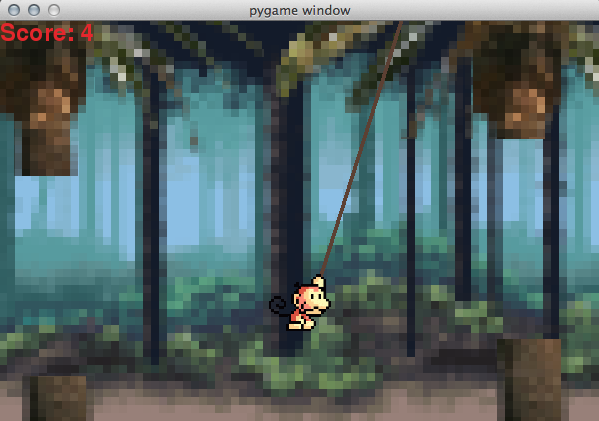
\includegraphics[width=0.48\textwidth]{figures/swingy}
        \label{fig:swingy}
    }\hfill
    \subfloat[SwingyMonkey State]{%
        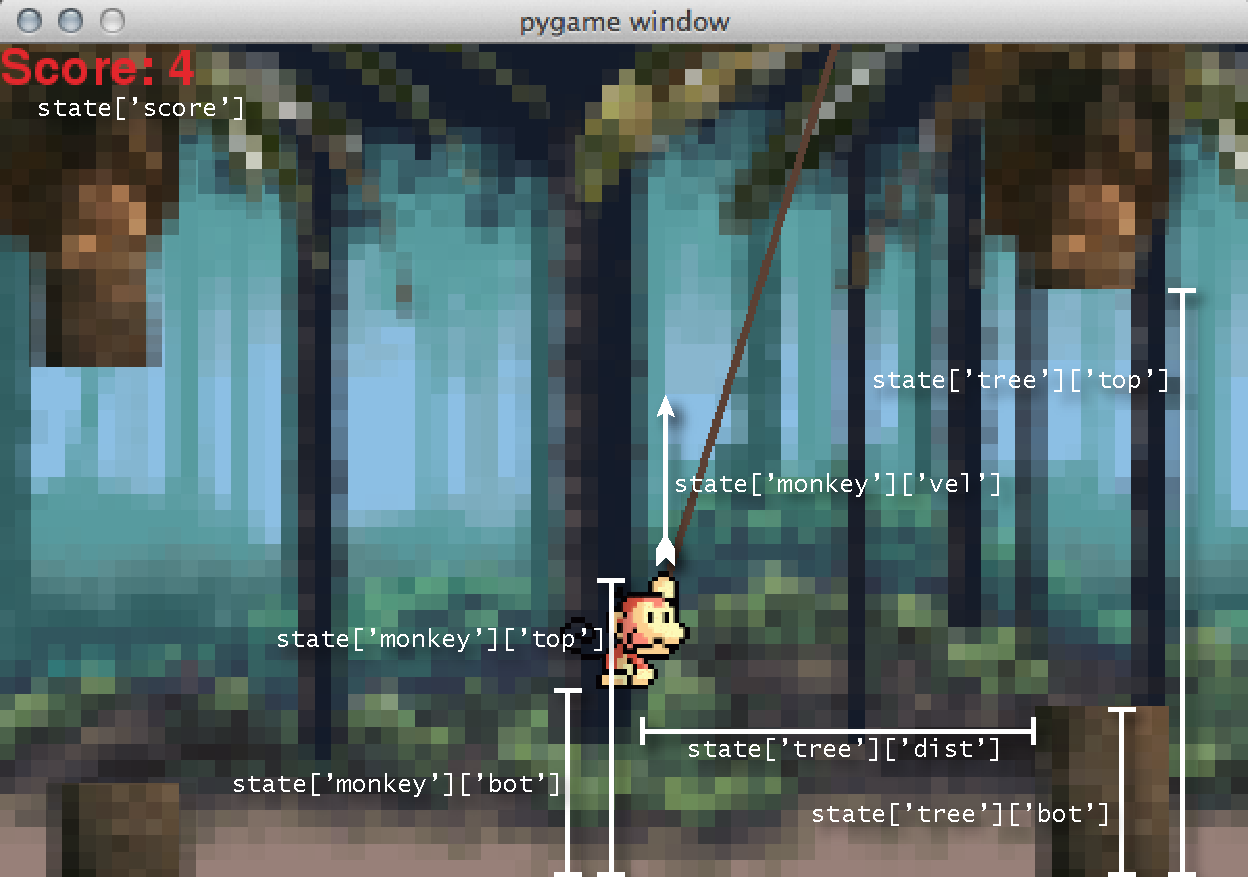
\includegraphics[width=0.48\textwidth]{figures/swingy-ann}
        \label{fig:swingy-ann}
    }
    \caption{(a) Screenshot of the Swingy Monkey game.  (b) Interpretations of various pieces of the state dictionary.}
\end{figure}

%%%%%%%%%%%%%%%%%%%%%%%%%%%%%%%%%%%%%%%%%%%%%%%%%%%%%%%%%%%%%%%%%%%%%%%%%%%%%%%%%%%%%%%%%%
\newpage
\textbf{Solution:}
My agent was able to consistently get large scores before the 100th epoch number, as shown in the table below. As my method of choice to increase performance, I decided to decay both the $\epsilon$ greedy-policy parameter and $\alpha$ learning rate over time. I used the following function for $\epsilon_t$.
\begin{equation*}
    \epsilon_t = \frac{1}{1 + \frac{1}{2} N(s) \epsilon_0}
\end{equation*}
Where $N(s)$ is the number of times an action has been taken from state $s$ and $\epsilon_0$ is the initial epsilon, a choice of hyper-parameter. I used the following function for $\alpha_t$.
\begin{equation*}
    \alpha_t = \frac{1}{1 + \frac{1}{20} N(s,a) \alpha_0}
\end{equation*}
Where $N(s, a)$ is the number of times the action $a$ has been taken from state $s$ and $\alpha_0$ is the initial alpha. This method combines two approaches I learned from section (where I learned to use $N(s)$ and $N(s,a)$) and \href{https://medium.com/analytics-vidhya/learning-rate-decay-and-methods-in-deep-learning-2cee564f910b}{this Medium blog post} (where I learned a method for decaying the learning rate (despite that the post decays using epoch number)). The choice of $1/2$ and $1/20$ was obtained by eye-balling the rate of decay and briefly experimenting.

To find my hyper-parameters, I searched in intervals of $0.2$ in the range $(0.1, 1)$. For computational purposes I decided to fix $\gamma = 0.9$ (which was suggested by a TF on Ed) and only search for the initial $\epsilon_0$ and $\alpha_0$ as I did not have time to search over $\gamma$. I ran each hyper-parameter combination for five histories and computed the maximum score for each history. I then averaged these maximum scores as well as their variances, which are reported in the table below. 
\begin{center}
\begin{tabular}{||c c c c c||} 
 \hline
 $\epsilon_0$ & $\alpha_0$ & Max Score & Mean Max Score & Variance of Max Scores\\ [0.5ex] 
 \hline\hline
 0.1 & 0.1 & 1392 & 1011.6 & 60223.04 \\ 
 \hline
 0.1 & 0.3 & 1387 & 1217 & 36797.2 \\
 \hline
 0.1 & 0.5 & 1073 & 904 & 14070 \\
 \hline
 0.1 & 0.7 & 859 & 761.6 & 6433.04 \\
 \hline
 0.1 & 0.9 & 1633 & 1049.2 & 112134.96 \\
 \hline
 0.3 & 0.1 & 1621 & 1037.6 & 101155.44 \\ 
 \hline
 0.3 & 0.3 & 1005 & 905.4 & 6616.64 \\
 \hline
 0.3 & 0.5 & 1058 & 634.0 & 240040 \\
 \hline
 0.3 & 0.7 & 843 & 773.4 & 2497 \\
 \hline
 0.3 & 0.9 & 1861 & 1151 & 255509.36 \\
 \hline
 0.5 & 0.1 & 1291 & 978.8 & 66869.36 \\ 
 \hline
 0.5 & 0.3 & 1172 & 914.8 & 31078.16 \\
 \hline
 0.5 & 0.5 & 1139 & 704.6 & 141217.04 \\
 \hline
 0.5 & 0.7 & 1200 & 968.200 & 24439.36 \\
 \hline
 0.5 & 0.9 & 1378 & 926.8 & 69152.56 \\
 \hline
 0.7 & 0.1 & 1461 & 965.6 & 132876.64 \\ 
 \hline
 0.7 & 0.3 & 1561 & 1080.4 & 124933.04 \\
 \hline
 0.7 & 0.5 & 1174 & 807.4 & 60172.24 \\
 \hline
 0.7 & 0.7 & 943 & 808.6 & 12146.64 \\
 \hline
 0.7 & 0.9 & 1205 & 1088.4 & 8107.04 \\
 \hline
 0.9 & 0.1 & 1148 & 857.6 & 33975.04 \\ 
 \hline
 0.9 & 0.3 & 1163 & 875.8 & 40055.36 \\
 \hline
 0.9 & 0.5 &  1158 & 881.4 & 41651.04 \\
 \hline
 0.9 & 0.7 & 1118 & 757.2 & 151257.36 \\
 \hline
 0.9 & 0.9 & 1851 & 1014.4 & 196285.84 \\
 \hline
\end{tabular}
\end{center}
As we can see, the variances are all very high. This may be due to only running $5$ histories: running more would potentially reduce this variance. Based on the values in this table, I decided to choose $\epsilon_0 = 0.1$ and $\alpha_0 = 0.9$. This choice had the highest max and mean score over the five histories. While the variance is high, I think the trade-off of an improved score is worth it.

My code is given below.
\begin{python}
# Imports.
import numpy as np
import numpy.random as npr
import pygame as pg
import matplotlib.pyplot as plt

# uncomment this for animation
# from SwingyMonkey import SwingyMonkey

# uncomment this for no animation
from SwingyMonkeyNoAnimation import SwingyMonkey


X_BINSIZE = 200
Y_BINSIZE = 100
X_SCREEN = 1400
Y_SCREEN = 900


class Learner(object):
    def __init__(self, _gamma = 0.9, _init_epsilon = 0.1, _init_alpha = 0.9):
        self.last_state = None
        self.last_action = None
        self.last_reward = None
        self.A = np.zeros((2, X_SCREEN // X_BINSIZE, Y_SCREEN // Y_BINSIZE))
        self.gamma = _gamma
        self.init_epsilon = _init_epsilon
        self.init_alpha = _init_alpha


        # We initialize our Q-value grid that has an entry for each action and state.
        # (action, rel_x, rel_y)
        self.Q = np.zeros((2, X_SCREEN // X_BINSIZE, Y_SCREEN // Y_BINSIZE))

    def reset(self):
        self.last_state = None
        self.last_action = None
        self.last_reward = None

    def discretize_state(self, state):
        """
        Discretize the position space to produce binned features.
        rel_x = the binned relative horizontal distance between the monkey and the tree
        rel_y = the binned relative vertical distance between the monkey and the tree
        """

        rel_x = int((state["tree"]["dist"]) // X_BINSIZE)
        rel_y = int((state["tree"]["top"] - state["monkey"]["top"]) // Y_BINSIZE)
        return (rel_x, rel_y)

    def action_callback(self, state):
        new_state = state
        sp = self.discretize_state(new_state)

        if self.last_state:
            s = self.discretize_state(self.last_state)
            a = self.last_action
            self.A[a, s[0], s[1]] += 1
            alpha = 1 / (1 + 0.05 * self.A[a, s[0], s[1]]) * self.init_alpha
            self.Q[a, s[0], s[1]] = self.Q[a, s[0], s[1]] + alpha * (self.last_reward + self.gamma * (np.max(self.Q[:, sp[0], sp[1]])) - self.Q[a, s[0], s[1]])
        
        new_action = 0
        epsilon = 1 / (1 + 0.5 * self.A[:, sp[0], sp[1]].sum()) * self.init_epsilon
        if npr.rand() < epsilon:
            # Take random choice of 0 or 1
            new_action = int(0.5 > npr.rand())
        else:
            # Take optimal action
            new_action = int(np.argmax(self.Q[:, sp[0], sp[1]]))

        self.last_action = new_action
        self.last_state = new_state

        return self.last_action

    def reward_callback(self, reward):
        """This gets called so you can see what reward you get."""

        self.last_reward = reward


def run_games(learner, hist, iters=100, t_len=100):
    """
    Driver function to simulate learning by having the agent play a sequence of games.
    """
    for ii in range(iters):
        # Make a new monkey object.
        swing = SwingyMonkey(sound=False,  # Don't play sounds.
                             text="Epoch %d" % (ii),  # Display the epoch on screen.
                             tick_length=t_len,  # Make game ticks super fast.
                             action_callback=learner.action_callback,
                             reward_callback=learner.reward_callback)

        # Loop until you hit something.
        while swing.game_loop():
            pass

        # Save score history.
        hist.append(swing.score)

        # Reset the state of the learner.
        learner.reset()
    pg.quit()
    return


if __name__ == '__main__':
    agent = Learner()
    hist = []
    run_games(agent, hist, 100, 0)
    print(hist)
\end{python}




%%%%%%%%%%%%%%%%%%%%%%%%%%%%%%%%%%%%%%%%%%%%%%%%%%%%%%%%%%%%%%%%%%%%%%%%%%%%%%%%%%%%%%%%%%

\newpage
\newpage
%%%%%%%%%%%%%%%%%%%%%%%%%%%%%%%%%%%%%%%%%%%%%
% Name and Calibration
%%%%%%%%%%%%%%%%%%%%%%%%%%%%%%%%%%%%%%%%%%%%%
\newpage
\subsection*{Name}
\subsection*{Collaborators and Resources}
Whom did you work with, and did you use any resources beyond cs181-textbook and your notes?

James Kitch, Julian Schmitt.

I consulted this Medium blog post which described a learning rate decay method: https://medium.com/analytics-vidhya/learning-rate-decay-and-methods-in-deep-learning-2cee564f910b. I combined this with an idea from section notes to come up with my functions for $\alpha_t$ and $\epsilon_t$.

\subsection*{Calibration}
Approximately how long did this homework take you to complete (in hours)? 
25 hours.
\end{document}